\documentclass[12pt]{article}
\usepackage[dvips]{epsfig}
\usepackage{color}
\usepackage{url}
\usepackage[colorlinks=true]{hyperref}

\begin{document}

\section*{GENESIS: Introduction}

{\bf Related Documentation:}
% start: userdocs-tag-replace-items related-workflow
% end: userdocs-tag-replace-items related-workflow

\section*{User Workflow Overview}

The relationship between experiment and simulation in computational neuroscience is illustrated in the figure below.  

 \begin{figure}[h]
    \centering
    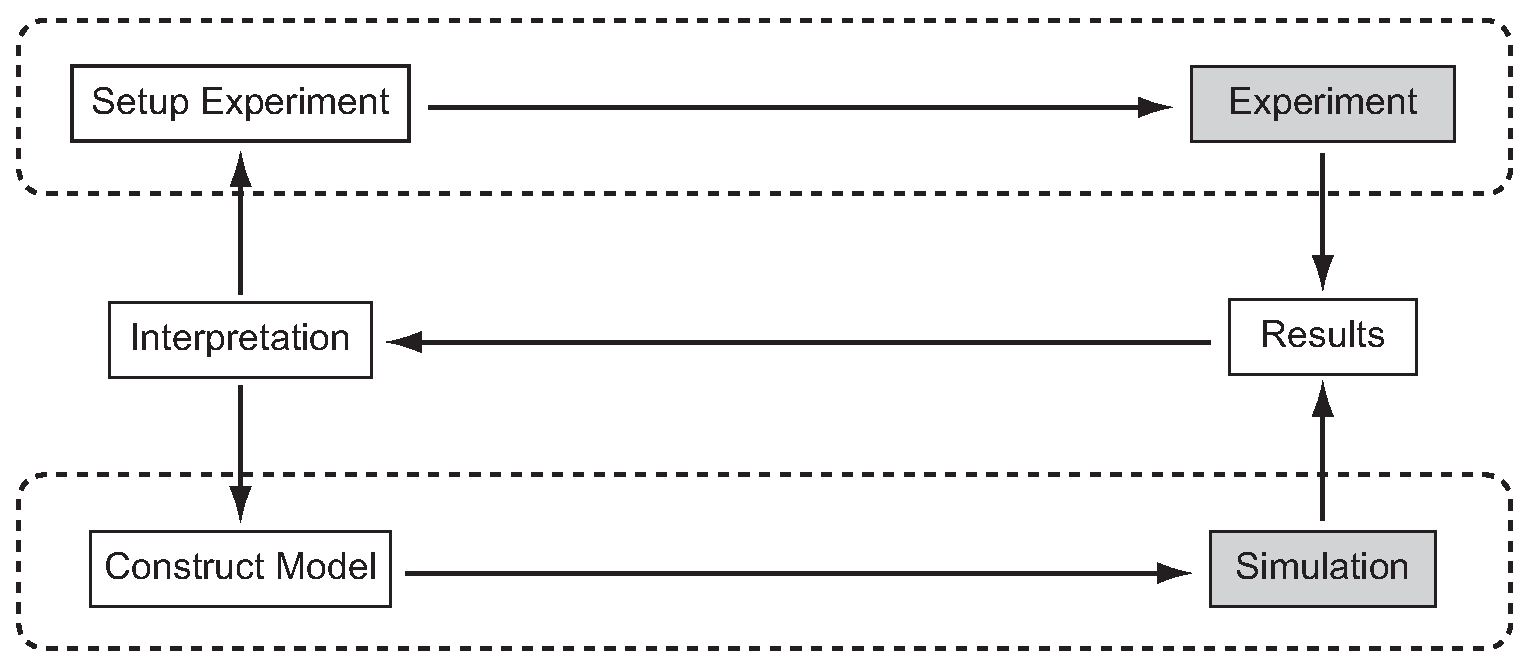
\includegraphics[scale=0.4]{figures/Exp-Sim-8.eps}
 %   \caption{{\bf A Dummy Figure:} Example of Latex code to incorporate
 %      a figure into documentation.}
    \label{fig:df-1}
 \end{figure}

Conducting experiments and running simulations are two iterative processes connected by a feedback loop that uses interpretation of results to design new experimental setups and model constructions. GENESIS supports the lower loop within the system as shown above.

\subsection*{GENESIS User Workflow}

The typical workflow within GENESIS has five basic steps, as the following figure illustrates. 
 \begin{figure}[h]
    \centering
    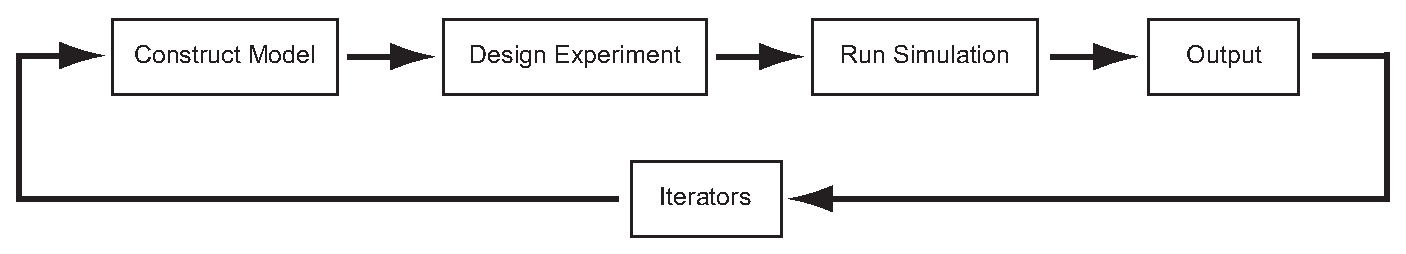
\includegraphics[scale=0.5]{figures/workflow.eps}
 %   \caption{{\bf A Dummy Figure:} Example of Latex code to incorporate
 %      a figure into documentation.}
    \label{fig:df-1}
 \end{figure}

This workflow provides an organizing principle that guides the user experience of GENESIS, for example, the \href{../gtube/gtube.tex}{\bf GUI} and tutorial documentation.

\begin{enumerate}

\item {\bf Construct model:} Simple models can be created directly within the {\bf G-Shell} by entering commands. More complex models can be imported into the {\bf G-Shell} from either the GENESIS model libraries or from external model libraries. The model can also be explored, checked, and saved.

\item {\bf Design experiment:}  Set model parameter values specific to a given simulation, the stimulus parameters for a given simulation run or  `experiment', and/or the variables to be stored for subsequent analysis.

\item  {\bf Run simulation:} Configure runtime options, check, run, reset simulation, and save model state. The model state can be saved at any simulation time step to allow it to be imported into a subsequent GENESIS session. Output is flushed to raw result storage for subsequent data analysis. 

\item {\bf Output:}  Check simulation output and the validity of results to determine whether simulation output exists in the correct locations. Output can be analyzed either within GENESIS or piped to external applications such as \href{http://www.mathworks.com/}{\bf Matlab}, \href{http://plasma-gate.weizmann.ac.il/Grace/}{\bf Grace}, or \href{http://www.wolfram.com/}{\bf Mathematica}.

\item {\bf Iterators:} Close the loop between output of results and model construction in the GENESIS users workflow. Iterators connect experimental results and model output and include for example, automated construction of simulations and batch files, static parameter searching, and active parameter searching using the dynamic clamp. 

\end{enumerate}

\end{document}